\documentclass[a4paper,oneside,hidelinks]{Tptesi2}
\usepackage{hyperref}
\usepackage[italian]{babel}
\usepackage{listings}
\usepackage{amsmath,amssymb}
\usepackage{verbatim}
\usepackage{indentfirst}
\usepackage[utf8]{inputenc}
\usepackage{subfigure}
\usepackage{algorithmic}
\usepackage{framed}
\usepackage{rotating}
\usepackage{cite}
\usepackage{minted}
\setminted{linenos,breakbytokenanywhere,breaklines,frame=lines}

% Packages -----------------------------------------------------------------------
%\usepackage{amsthm}
%\usepackage{amsmath}          % Non necessario se usi TPTESI2 perche' gia` incluso
%\usepackage[dvips]{graphicx}  % Non necessario se usi TPTESI2 perche' gia` incluso
%\usepackage{url} %non usare se si usa hyperref


\newcommand{\mr}{\emph{motore di ricerca}}
\newcommand{\Mr}{\emph{Motore di ricerca}}
\newcommand{\ws}{Web~service }


% Use a small font for the verbatim environment
\makeatletter  % makes '@' an ordinary character
\renewcommand{\verbatim@font}{%
  \ttfamily\footnotesize\catcode`\<=\active\catcode`\>=\active%
}
\makeatother   % makes '@' a special symbol again
%
% Simboli Matematici -------------------------------------------------------------
%\newcommand{\h}{\mathcal{H}_\infty} % scorciatoia per sequenza usata spesso
% Definizioni & Teoremi ----------------------------------------------------------
\newtheorem{teorema}{Teorema}[chapter]
\newtheorem{corollario}[teorema]{Corollario}
\newtheorem{lemma}[teorema]{Lemma}
%\theoremstyle{definition}
\newtheorem{definizione}{Definizione}[chapter]
\newtheorem{proposizione}[definizione]{Proposizione}
% Formattazione Figure -----------------------------------------------------------
\setcounter{topnumber}{3}
\setcounter{totalnumber}{3}
\def\topfraction{1}
\def\textfraction{0}
% Fuzz ---------------------------------------------------------------------------
%\hfuzz10cm %Non scassare linee che escono dal bordo
% Frontespizio -------------------------------------------------------------------
       \title{Riconoscimento di azioni in video calcistici usando reti neurali ricorrenti}
       \author{Alberto Baldrati}
       \titolocorso{Ingegneria Informatica}
       \chair{Marco Bertini }
       \numberofmembers{1} %numero dei relatori
       \degreeyear{2018/2019}
  

%
% ---- Inclusioni (vedi piu` sotto per il comando "include" --------------
%\includeonly {introduzione,chapter1, chapter2}
%\includeonly {chapter1, chapter2, chapter3, chapter4, chapter5, chapter6}
%\includeonly{chapter6}
%
\hypersetup{%
%  pdfpagemode=FullScreen,%
  plainpages=false,%
  breaklinks,%
  pdftitle={},%
  pdfauthor={},%
  pdfsubject={},%
  pdfkeywords={},%
  colorlinks=false}

\begin{document}

\frontmatter

%\hyphenation{}
%
\pagestyle{headings} % rende attive le impostazioni sulla testata!
%
\maketitle % crea il frontespizio (ricordati di copiare "stemma.eps" nella tua directory)
%
%
%\pagenumbering{roman}
\tableofcontents % inserisce indice generale
\cleardoublepage
%\addcontentsline{toc}{chapter}{Elenco delle figure}
%\listoffigures   % inserisce indice figure
%\addcontentsline{toc}{chapter}{Elenco delle tabelle}
%\listoftables    % inserisce indice tabelle
%\addcontentsline{toc}{chapter}{Elenco degli algoritmi}
%\listofalgorithms
%
%--------------- Inizio del testo vero e proprio
%

%\cleardoublepage
%\pagenumbering{arabic}
%RINGRAZIAMENTI
\frontmatter
\chapter{Introduzione}\label{ch:introduzione}
\section*{Motivazioni}
In Italia e nel mondo lo sport, il calcio in particolare, ha una grande importanza sociale e culturale.
\\A causa di questa importanza e del numero di appassionati, lo sport professionistico è un settore in cui vengono effettuati grandi investimenti e nel quale vengono spesi annualmente miliardi di euro, ad esempio i diritti televisivi di serie A per il triennio 2018-2021 sono stati venduti dalla Lega Calcio a oltre \textbf{1.4 miliardi} di euro l'anno. \cite{DirittiTriennio2018-21}
\\Non sorprenderà quindi che una buona percentuale dei soldi che entrano nelle casse dei club calcistici è data prorio dai sopracitati diritti, sempre in serie A nel 2015/2016 tale percentuale era mediamente il \textbf{48\%}. \cite{impattoDirittiTv}
\\I broadcaster televisivi, spendendo per tali diritti così tanti soldi e mirando ovviamente a effettuare del profitto, devono avere un gran numero di abbonati. Per raggiungere tale obbiettivo essi offrono servizi di qualità, come ad esempio studi pre/post partita, approfondimenti, ma sopratutto \textbf{highlights} che vanno a riassumere i momenti salienti di una partita. 
\\La creazione di quest'ultimi può sembrare un'operazione banale e infatti lo è, tuttavia richiede che una persona annoti manualmente le azioni pericolose e in particolare i goal.
\\Questo procedimento dovendo essere ripetuto per tutte le partite rappresenta un costo non indifferente per i suddetti broadcaster, che avrebbero un grande interesse ad automatizzare il procedimento.
\section*{Presentazione del lavoro}
In questo elaborato di tesi, partendo dal lavoro di \citet{soccerNet} , verrà descritta una tecnica di automatizzazione del problema citato in precedenza, la quale tuttavia non genera veri e propri highlights, i quali includerebbero oltre ai goal anche azioni pericolose e momenti salienti della partita, ma isola durante l'arco di una partita tre tipi di azione: i \textbf{cartellini}, le \textbf{sostituzioni} ed i \textbf{goal}.
\\Il lavoro descritto è suddiviso in due parti, la prima parte consiste in un problema di \textbf{classificazione} in cui si è proceduto ad addestrare una rete neurale, nella seconda è stata usata la medesima rete neurale precedentemente addestrata per isolare le azioni di nostro interesse.
\\Il Dataset su cui abbiamo lavorato è formato da \textbf{500} partite prese dai maggiori campionati europei.




\mainmatter
\chapter{Metodo}\label{ch:chapter1}
\section{Features}
Per ulteriori dettagli su come sono state processate le features fare riferimento a \citep{soccerNet}
\subsection{Preparazione dei video }
Prima di procedere con l'estrazione delle \textbf{features} mediante una rete neurale, sono state effettuate sui video le seguenti operazioni:
\begin{itemize}
\item Sono stati \textbf{tagliati} in modo che l'inizio del video coincida con l'inizio della partita
\item Dalla risoluzione \textbf{HD} sono stati portati ad una risoluzione di \textbf{224 x 224}
\item Sono stati unificati a \textbf{25fps}
\end{itemize}
Tale rappresentazione garantisce video compatibili con l'estrazione di features mediante reti neurali e permette di mantenre un dataset di dimensioni accettabili.
\subsection{Estrazione delle features}
Dopo aver processato i video come descritto sopra si è passati poi alla estrazione delle features.
\\Per tale operazione è stata utilizzata la rete neurale convoluzionale profonda (ConvNet) \textbf{ResNET}, essa data un immagine (nel nostro caso un frame del video) in input, ha come output, al layer \textit{fc1000}, \textbf{2048} features.
\\In particolare è stata usata la variante \textbf{ResNet-152} preallenata sul dataset \textbf{ImageNet}.
\\Dato che tale rete neurale è applicata sui singoli frame, essa non mantiene intrinsecamente informazioni temporali, a causa di ciò essa è stata utilizzata per estrarre features ogni \textbf{0.5} secondi, preocupandosi successivamente di mantenerle nell'ordine corretto.
\\Per ridurre le dimensioni delle features è stata infine applicata la \textbf{Principal Component Analaysis} (\textbf{PCA}) che riduce il numero di features per frame da \textbf{2048} a \textbf{512} mantenendo il \textbf{93.9\%} della varianza.

\section{Pooling neural network}
Nel paper di \citet{soccerNet} vengono testate varie tipologie di pooling, le quali hanno in comune la sigmoide come funzione di attivazione nell'ultimo layer per permettere annotazioni multiple in un singolo campione.
Le varie tipologie di pooling utilizzate sono: \textbf{mean}, \textbf{max}, \textbf{CNN}, \textbf{SoftDBOW}, \textbf{NetFV}, \textbf{NetVLAD} e \textbf{NetRVLAD}. \cite{MiechPooling}
\\Vedremo successivamente che il modello che ottiene i risultati migliori è il \textbf{NetVLAD}, avente il \textit{fully connected layer} di uscita con un \textit{dropout rate} pari a \textbf{0.4} per cercare di prevenire l'\textit{overfitting}.

\section{GRU-model}
\label{section : grumodel}
Il modello migliore da me sviluppato è una \textbf{rete neurale ricorrente} (\textbf{RNNs}) basata su \textbf{GRU} layer (\textbf{Gated Recurrent Unit}). 
\\Più nel dettaglio, come si può notare dal codice sottoriportato, l'intero modello è costituito proprio da \textbf{tre} layer di tipo GRU e dal layer di \textbf{output}.
\\I tre layer GRU sono stati usati in modo \textbf{bidirezionale} in quanto spesso ciò che avviene \textbf{dopo} un goal, un cartellino o una sostituzione \textbf{caratterizza} l'azione tanto quanto ciò è avvenuto \textbf{prima}, aiutando la rete neurale a classificare in modo corretto l'azione. Per tali layer la funzione di attivazione scelta è stata la \textit{rectified linear unit} (\textbf{ReLU}). \cite{DeepLearningPython}
\\Il layer di output, come in tutti i problemi di machine learning, è strettamente collegato al tipo di problema che si deve fronteggiare. Il nostro, almeno nella fase iniziale, è un problema di classificazione binaria avente \textbf{quattro} classi (background, cartellino, sostituzione e goal), per questo motivo tale layer come funzione di attivazione la \textbf{sigmoide} ed ha esattamente \textbf{4} neuroni.
\\Tale modello è stato realizzato con la libreria \textbf{Keras} \cite{chollet2015keras}, usando come \textit{backend} \textbf{TensorFlow} \cite{tensorflow2015-whitepaper}
\begin{minted}[baselinestretch=1, fontsize=\footnotesize]{python}
model = Sequential()
model.add(layers.Bidirectional(layers.GRU(512,
                                          activation='relu',
                                          dropout=0.1,
                                          recurrent_dropout=0.4,
                                          return_sequences=True,
                                          ),
                               input_shape=(None, 512))
          )

model.add(layers.Bidirectional(layers.GRU(256,
                                          activation='relu',
                                          dropout=0.1,
                                          recurrent_dropout=0.4,
                                          return_sequences=True,
                                          )
                               )
          )

model.add(layers.Bidirectional(layers.GRU(128,
                                          activation='relu',
                                          dropout=0.1,
                                          recurrent_dropout=0.4,
                                          )
                               )
          )

model.add(layers.Dense(4,
                       activation='sigmoid')
          )
\end{minted}
Si può notare come siano stati utilizzati dei \textit{dropout layer} per cercare di ridurre il problema dell'overfitting, essi sono stati usati sia nella versione \textbf{standard}, sia nella versione apposita per le \textbf{reti neruali ricorrenti}, la quale utilizza la medesima \textit{dropout mask} ad ogni \textit{timestamp} permettendo di propagare l'errore in modo corretto. \cite{DeepLearningPython}
\\Come otimizzatore è stato utilizzato \textbf{RMSProp} con il \textbf{learning rate} di default (\textbf{lr$=$0.001}), era tuttavia presente una \textit{callback} che in caso di non miglioramento del modello per più di dieci epoche lo riduceva di un fattore 0.4.
\\La \textit{loss function} utilizzata, essendo un problema di classificazione binaria multiclasse, è la \textbf{binary crossentropy}.
\chapter{Esperimenti Classificazione}\label{ch:chapter2}
\section{Dataset}
\subsection{Descrizione del dataset }
Il Dataset su cui sono stati effettuati gli esperimenti descritti in questo elaborato di tesi è il medesimo usato da \citet{soccerNet}.
Tale Dataset è formato da \textbf{500 partite}, per un totale di \textbf{764 ore} di gioco, prese dai principali campionati europei durante le tre stagioni 2014-2015, 2015-2016 e 2016-2017.
\\Maggiori dettagli sui campionati e sulla suddivisone delle partite sono foriniti nella tabella \textbf{\ref{table: Dataset}}
\\Per assicurare un corretto confronto con la baseline, ho utilizzato la medesima suddivione utilizzata nel loro \textit{paper} \cite{soccerNet} nella quale le partite del dataset sono state suddivise in modo casuale in raggruppamenti di \textbf{300}, \textbf{100}, \textbf{100} rispettivamente per \textbf{training}, \textbf{validation} e \textbf{testing}, assicurandosi in questo modo una distribuzione similare degli eventi in ogni porzione di dataset.
\begin{table}[H]
\caption{Suddivisone delle partite per lega e anno nel nostro Dataset}
\centering
\begin{tabular}{c| | c|c|c | | c}
\multicolumn{1}{c}{}&\multicolumn{3}{c}{Stagioni}& \\
Lega & 14/15 & 15/16 & 16/17 & \textbf{Total} \\
\hline
EN - EPL & 6 & 49 & 40 & \textbf{95} \\
ES - LaLiga & 18 & 36 & 63 & \textbf{117} \\
FR - Ligue 1 & 1 &  3 & 34 & \textbf{38} \\
DE - BundesLiga & 8 & 18 & 27 & \textbf{53} \\
IT - Seria A & 11 & 9 & 76 & \textbf{96} \\
EU - Champions & 37 & 45 & 19 & \textbf{101} \\
\hline
Total & \textbf{81} & \textbf{160} & \textbf{259} & \textbf{500} \\ [1ex]

\end{tabular}
\label{table: Dataset}
\end{table}
Dai video delle partite sono state poi estratte le features mediante la rete neurale ResNET con il procedimento descritto in precedenza.
\subsection{Label}
Oltre ai video, il Dataset è formato dalle \textbf{annotazioni} (\textbf{label}), le quali sono state inizialmente ottenute effetuando il \textit{parsing} dei report delle partite direttamente sui siti delle varie leghe calcistiche.
\\Tuttavia la granularità delle annotazioni così ottenute non è abbastanza elevata per i nostri propositi essendo di un \textbf{minuto}, a causa di ciò si sono dovuti riannotare \textbf{manualmente} gli eventi, all'interno del minuto già noto, per ottenere una precisione di un \textbf{secondo}.
\\Per essere in grado di fare ciò, si sono dovuti definire gli esatti istanti temporali che corrispondono alle azioni di nostro interesse.
\\Definiamo quindi:
\begin{itemize}
\item L'evento \textbf{Goal} come l'istante in cui la palla oltrepassa la linea di porta
\item L'evento \textbf{Cartellino} come l'instante in cui l'arbitro estrae il cartellino
\item L'evento \textbf{sostituzione} l'istante come in cui il giocatore entra nel terreno di gioco
\end{itemize}
L'unica eccezione alle definizioni sovracitate sono le sostituzioni avvenute durante l'\textbf{intervallo}, per le quali è impossibile dare una definzione che corrisponda con quanto accade in video.
\subsection{Suddivisone minuto per minuto}
Il nostro dataset formato, come detto sopra, da 500 partite e 764 ore di video, è stato poi suddiviso in porzioni disgiunte aventi la \textbf{durata di un minuto} per poter essere elaborato da un rete neurale.
\\In questa fase il nostro è un problema di \textbf{classificazione}, in cui un singolo campione è formato da \textbf{120 raggruppamenti} di features ed è annotato con gli eventi occorrenti in quel minuto.
\\Ovviamente essendo molto più probabile che in un minuto di una partita non accada niente piuttosto che sia presente un'azione da noi ricercata, il nostro dataset è decisamente \textbf{sbilanciato}, esso infatti nel training set contiene:
\begin{itemize}
\item \textbf{1246} campioni in cui è presete un \textbf{cartellino}
\item \textbf{1558} campioni in cui è prsente una \textbf{sostituzione}
\item \textbf{960} campioni in cui è presente un \textbf{goal}
\item \textbf{23750} campioni di \textbf{background}, ovvero in cui non avviene nessuna delle tre azioni sopracitate
\end{itemize}
È importante notare inoltre come ben \textbf{115} campioni abbiano label multiple, per una corretta classificazione è necessario quindi che il modello sviluppato ammetta la possbilità di classificare questi campioni nel modo corretto.
\section{Metriche}
\subsection{Mean Average Precision}
La metrica usata nel paper di riferimento con cui ci andremo a confrontare, nel task di \textbf{classificazione}, è la metrica denominata \textbf{Mean Average Precision} (\textbf{mAP}). Per il calcolo di tale metrica viene utilizzata la \textbf{precision-recall curve}.
\\Prima di procere oltre è bene introdurre i concetti di \textbf{precision} e \textbf{recall}:
\begin{itemize}
\item La metrica \textbf{precison} misura quanto accurate sono le predizioni, ovvero la precentuale di previsioni corrette.
\begin{equation}
Precision=\frac{True Positives}{True Positives + False Positives}
\label{Precision}
\end{equation}
\item La metrica \textbf{recall} misura quanto correttamente si riesce a trovare tutti i positivi, può essere pensata quindi come l'abilità di un modello di trovare i punti di interesse di un dataset.
\begin{equation}
Recall=\frac{True Positives}{True Positives + False Negatives}
\label{Recall}
\end{equation}
\end{itemize}
La metrica \textbf{Average-Precision} (\textbf{AP}) è defnitita come l'area al di sotto della curva precision-recall.
\\Infine la metrica \textbf{Mean Average Precision} è definita come la \textbf{media} tra i valori delle \textbf{AP} per ogni evento. 
\\Nel nostro caso quindi sono state calcolate \textbf{tre} AP (per \textbf{goal}, \textbf{sostituzioni} e \textbf{cartellini}) e successivamente ne è stata calcolata la media aritmetica.
\\Sfortunatamente non mi è stato possibile utilizzare tale metrica in fase di training (e quindi validazione), questo a causa del fatto che la \textbf{mAP} non è nativamente supportata in Keras, per poterla utilizzare è stato quindi necessario importare tale metrica da \textbf{Tensorflow}.
\\Le metriche di Tensorflow \textbf{non supportano} tuttavia i dati costruiti mediante \textbf{funzioni generatrici}, fatto invece necessario a causa della pesantezza dei nostri dati.
\\Per questo motivo per effettuare il \textit{fine-tuning} della mia rete neurale è stato necessario utilizzare una metrica diversa.
\subsection{F1}
La metrica utilizzata in fase di validazione è stata quindi la \textbf{F1}, essa combina le metriche di \textbf{Precision} e \textbf{Recall} sopra definite ed ha la seguente espressione:
\begin{equation}
F1=2*\frac{Precision * Recall}{Precision + Recall}
\label{F1}
\end{equation}
Nel nostro caso, dato che a noi interessa principlamente indivduare le porzioni di partita in cui accade un evento saliente, tale metrica è stata calcolata solamente sulle \textbf{tre} label di nostro interesse \textbf{trascurando} quella di background.
\\La metrica \textbf{F1} è stata inoltre utilizzata nel capitolo \ref{ch:chapter3} nel task di \textbf{localizzazione}
\section{Baseline}
I \textbf{risultati} ottenuti dalla baseline mediante le varie tecniche di pooling precedentemente accennate ed utilizzando le features estratte con ResNET sono elencati di seguito.\cite{soccerNet} 
\\Inizialmente sono stati effettuati degli esperimenti con i metodi di pooling senza effettuare alcun tipo di fine-tuning, in particolare sui metodi proposti da \citet{MiechPooling} (\textbf{SoftDBOW}, \textbf{NetFV}, \textbf{NetVLAD} e \textbf{NetRVLAD}) sono stati usati \textbf{k$=$64} cluster.
\\I risultati sono riassunti nella tabella \textbf{\ref{table: baselinek16}}.
\begin{table}[ht]
\caption{Risultati per i diversi metodi di pooling}
\centering
\begin{tabular}{c| | c}
\textbf{Pooling} & \textbf{mAP} \\
\hline
\textbf{Mean Pool.} & 40.2 \\
\textbf{Max Pool.} &  52.4\\
\textbf{CNN} & 53.5\\
\textbf{SoftDBOW} & 48.9\\
\textbf{NetFV} & 64.4\\
\textbf{NetRVLAD} & \textbf{65.9}\\
\textbf{NetVLAD} & 65.2\\ [1ex]

\end{tabular}
\label{table: baselinek16}
\end{table}
\\Ovviamente all'aumentare dei cluster aumenta la potenza espressiva del sistema, generando con buona probabilità un aumento di prestazioni.
\begin{table}[ht]

\caption{mAP al variare del numero di cluster k per i metodi di pooling proposti da \citet{MiechPooling}}
\label{table: baselinek16to512}
\centering
\begin{tabular}{c| | c|c|c |  c}
&\multicolumn{4}{c}{\textbf{Metodi di Pooling}} \\
k & \textbf{SoftBOW} & \textbf{NetFV} & \textbf{NetRVLAD} & \textbf{NetVLAD} \\
\hline
\textbf{16}& 54.9 & 63.0 & 64.4 & 65.2 \\
\textbf{32} & 57.7 & 64.0 & 63.8 & 65.1 \\
\textbf{64}& 58.8 &  64.1 & 65.3 & 65.2 \\
\textbf{128}& 60.6 & 64.4 & 67.0 & 65.6 \\
\textbf{256}& 61.3 & 63.8 & 67.7 & 67.0 \\
\textbf{512} & 62.0 & 62.1 & 67.4 & \textbf{67.8} \\[1ex]

\end{tabular}
\end{table}
\\Nella tabella \textbf{\ref{table: baselinek16to512}} infatti si vede come, inizialmente, all'aumentare delle dimensioni dei cluster migliorino le prestazioni, tuttavia oltre i 256 cluster esse iniziano a stabilizzarsi a causa dell'\textbf{overfitting}.
\\Inoltre la \textbf{complessità computazionale} cresce \textbf{linearmente} col numero dei cluster.\\
\linebreak
Il miglior risultato della baseline, quello quindi con cui ci siamo andati a confrontare, è ottenuto mediante \textbf{NetVLAD} con \textbf{k=512} cluster.
\\Come evidenziato nella tabella \textbf{\ref{table: baselinek16to512}} tale modello sul nostro dataset ha una mAP del \textbf{67.8\%}.
\section{I miei risultati}
Il modello che è stato utlizzato per cercare di migliorare i risultati ottenuti con la baseline, è stato precedentemente descritto nei dettagli.
\\Si tratta di una rete neurale ricorrente formata da tre layer GRU bidirezionali con l'aggiunta del layer di ouput.
\subsection{Training and Validation}
Come detto in precedenza a causa dell'incompatibilità tra le metriche di Tensorflow e i dati costruiti mediante generatori in Keras non mi è stato possibile  utilizzare la metrica mAP in fase di training del mio modello.
\\Per questo motivo nel grafico in figura \textbf{\ref{figure : trainingvalf1}} viene rappresentato l'andamento della metrica \textbf{F1}.
\\Nella figura \textbf{\ref{figure : trainingvalloss}} possiamo vedere come la loss function inizi a crescere dopo circa \textbf{10} epoche, facendoci pensare che il modello da li in poi inizi a peggiorare a causa dell'overfitting.
\\Tuttavia nella figura \textbf{\ref{figure : trainingvalf1}} possiamo vedere come la metrica f1 continui a migliorare anche dopo 10 epoche, stabilizzandosi circa alla trentsima epoca e avendo il miglior risultato all'epoca numero \textbf{34}.
\\Questa discrepanza è dovuta alla \textbf{polarizzazione}, verso 0 o verso 1, delle probabilità di output del mio modello.
\begin{figure}[ht]
\centering
\caption{Training and validation loss}
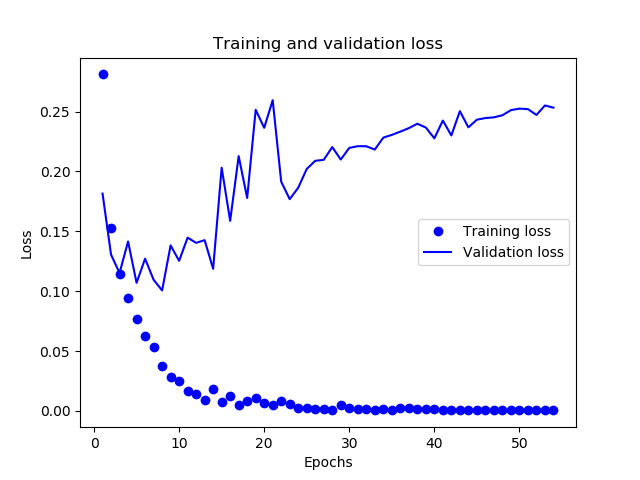
\includegraphics[width=\linewidth]{img/training-validation-loss.png}
\label{figure : trainingvalloss}
\end{figure}
\begin{figure}[H]
\centering
\caption{Training and validation F1}
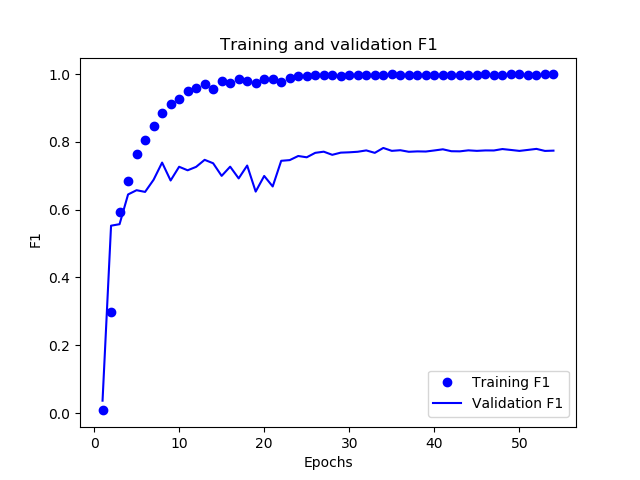
\includegraphics[width=\linewidth]{img/training-validation-F1.png}
\label{figure : trainingvalf1}
\end{figure}
\subsection{Test}
Per verificare definitivamente la bontà del mio modello è stato necessario testarlo sulla porzione di dataset riservata a tali propositi. 
\\In questa fase la metrica di riferimento torna a essere la \textbf{mAP}.
\begin{table}[ht]
\label{table: test}
\caption{Risultati sul test set}
\centering
\begin{tabular}{c|c|c||c}
\multicolumn{3}{c}{\textbf{AP}}\\
\textbf{Cartellino} & \textbf{Sostituzione} & \textbf{Goal} & \textbf{mAP} \\
\hline
77.6& 78.7 & 82.8 & \textbf{79.7} \\ [1ex]
\end{tabular}
\end{table}
\\Considerando che il risultato migliore della baseline contro cui mi sono confrontato è del \textbf{67.8\%}, il 
risultato ottenuto possiamo ritenerlo soddisfacente, essendo infatti un miglioramento di oltre il \textbf{10\%}.
\chapter{Conclusioni}\label{ch:conclusioni}
\section{Cosa ha funzionato bene}
Il lavoro che è stato descritto in questo elaborato di tesi può essere ritenuto soddisfacente.
\\Avendo infatti come punto di partenza il \textit{paper} \cite{soccerNet} in cui venivano effettuati esperimenti analoghi a quelli effettuati da me nel mio elaborato di tesi, sono riuscito mediante l'uso di reti neurali ricorrenti ad ottenere, nel task di classificazione, risultati persino migliori.
\\In tale task infatti siamo passati da una mAP del\textbf{ 67.8\%}, ottenuta nel sopracitato \textit{paper} grazie al metodo di pooling \textbf{netVLAD}, ad una mAP del \textbf{79.7\%} ottenuta grazie all'utilizzo di \textbf{reti neurali ricorrenti}.
\\Successivamente ci siamo spinti oltre, infatti siamo passati dal task di \textbf{classificazione} a quello di \textbf{localizzazione}, questo è stato possibile grazie ad un elaborazione del dataset con un meccanismo di \textit{sliding windows}.
\\Infine è stata inoltre descritta la procedura di generazione degli highlights, la quale, utilizzando la rete neurale addestrata nel task di classificazione, ha ottenuto nel task di \textbf{spotting} un \textbf{average-F1 score} del \textbf{83.5\%}
\section{Cosa ha funzionato meno bene}
\subsection{Data Augmentation}
Durante la fase di training, per cercare di ridurre gli effetti negativi dovuti al dataset fortemente sbilanciato, si è provato a usare una tecnica di \textbf{Data Augmentation}.
\\La nostra applicazione di tale tecnica è stata utilizzata per moltiplicare i campioni di ogni evento; questo è stato possibile anche in questa situazione mediante un meccanismo di \textbf{sliding-windows}.
\\Questi ulteriori campioni sono stati aggiunti poi al dataset, aiutando a risolvere lo sbilanciamento di quest'ultimo.
\\I risultati ottenuti applicando questa tecnica non sono stati tuttavia soddisfacenti, infatti le prestazioni della rete neurale si sono rivelate peggiori rispetto al modello che non ha fatto uso di \textbf{Data Augmentation}.
\subsection{Malfunzionamenti}
La rete neurale da me sviluppata non è ovviamente \textbf{immune} da \textbf{errori}, in particolare, come evidenziato dai risultati ottenuti sia nel task di localizzazione che in quello di classificazione, l'azione che viene identificata con risultati peggiori è quella che corrisponde all'estrazione di un cartellino.
\\Nella figura \textbf{\ref{figure : fakecard}} abbiamo un esempio di tale \textbf{malfunzionamento}, infatti in tale figura vediamo come l'inquadratura \textbf{in primo piano} dell'arbitro induca la nostra rete neurale a pensare che sia stato estratto un \textbf{cartellino}, quando invece il giocatore è stato richiamato solo \textbf{verbalmente}.
\begin{figure}[H]
\centering
\caption{Visualizzazione di un cartellino non correttamente predetto}
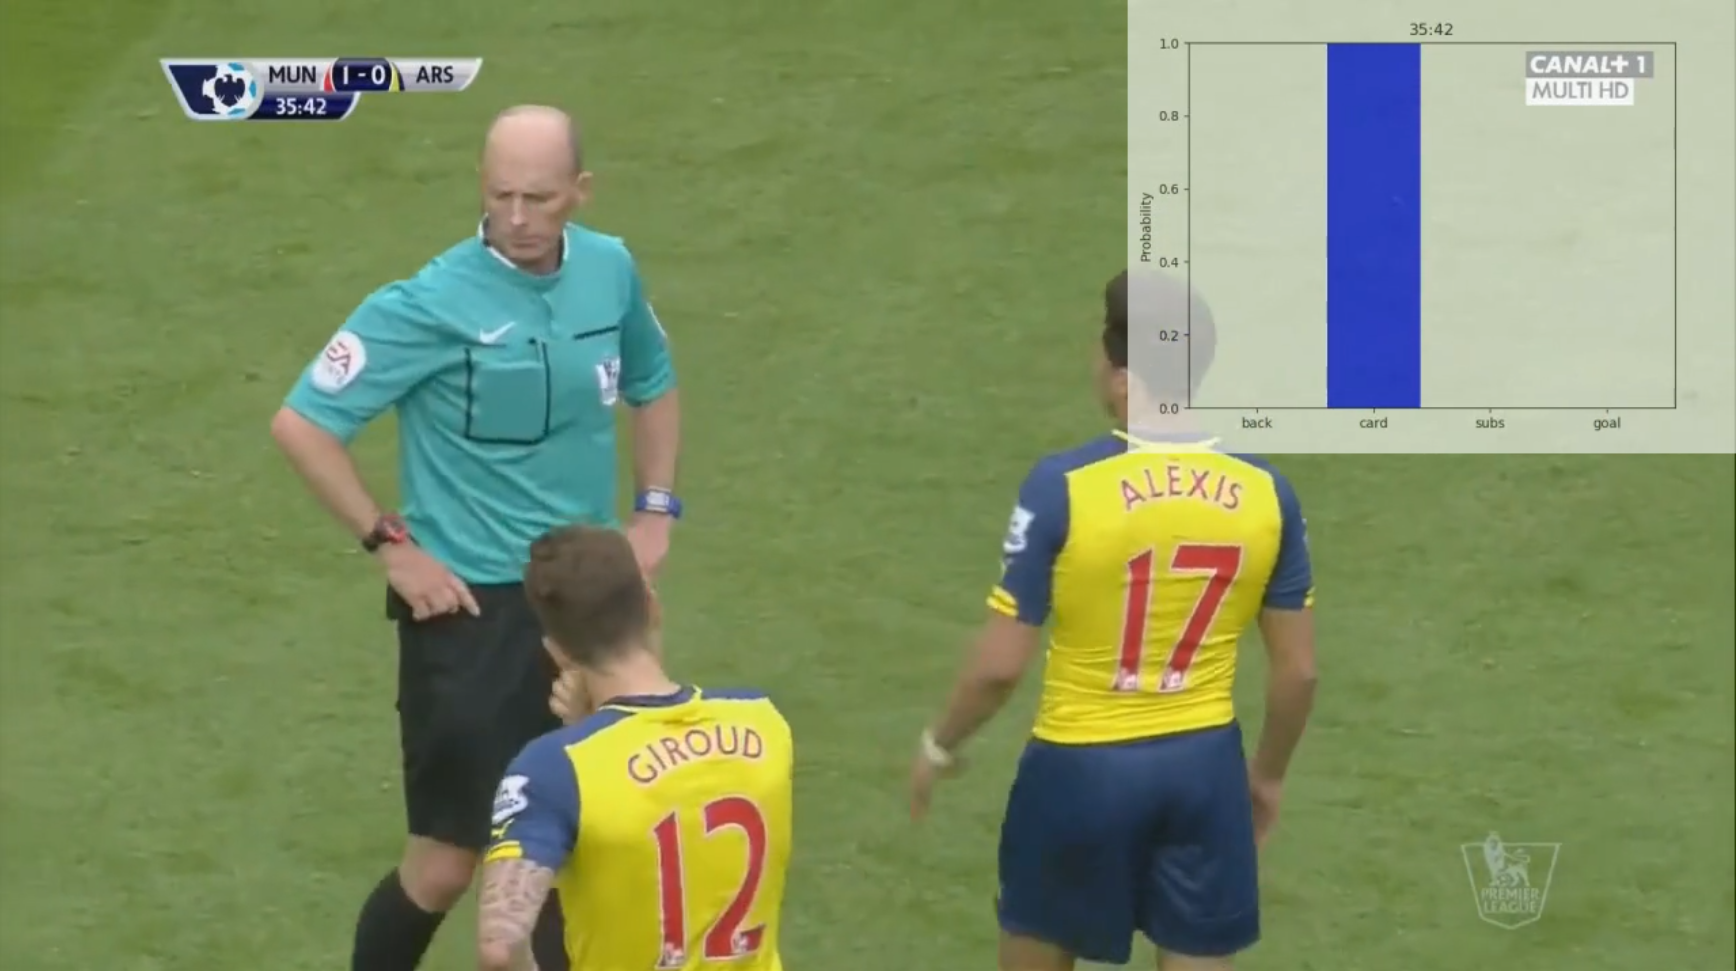
\includegraphics[width=\linewidth]{img/fakecardHQ.png}
\label{figure : fakecard}
\end{figure}
\section{Sviluppi futuri}
La naturale evoluzione di questo elaborato di tesi è quella di cercare di individuare \textbf{altre} tipologie di azioni oltre alle tre già prese in considerazione, ad esempio si potrebbero ricercare \textbf{tiri in porta}, \textbf{calci d'angolo} o \textbf{calci di rigore}.
\\Inoltre come citato nel \textit{paper} \citep{soccerNet}, nell'estrazione delle features non è stato preso in considerazione l'audio, presente invece nei video originali.
\\Indubbiamente esso aggiunge \textbf{informazioni significative} e potrebbe essere d'aiuto ai nostri scopi, tuttavia come ben sappiamo l'audio non è sempre strettamente collegato a ciò che accade in campo, ma dipende da altri fattori quali: squadra di casa, momento della partita, affluenza di pubblico allo stadio.
\\Questi fattori potrebbero \textit{confondere} la rete neurale, portando ad un peggioramento delle prestazioni.
\\Rimane impossibile quindi esprimersi a \textbf{priori} su un possibile aiuto dell'audio nell'addestramento della rete neurale.


\addcontentsline{toc}{chapter}{Bibliografia}
\bibliographystyle{plain}
\bibliography{files/biblio}
\bibliographystyle{unsrt}
%\bibliography{sp,xml}

\end{document} 